% =============================================================
%  Chapitre 1 — Contexte général du projet
% =============================================================
\chapter{Contexte général du projet}

\section{Introduction}

Le secteur des télécommunications traverse une période de transformation
rapide, et les entreprises qui y opèrent subissent une pression constante
pour valider leurs équipements réseau avec plus de rapidité, de fiabilité
et de rigueur. Les méthodes classiques de gestion des tests --- connexions
Telnet manuelles, procédures non standardisées, résultats stockés dans des
tableurs éparpillés --- montrent leurs limites face aux contraintes des
environnements industriels d'aujourd'hui. Dans ce contexte, livrer
rapidement des firmwares validés tout en garantissant traçabilité et
fiabilité n'est plus un avantage~: c'est une nécessité.

Ce projet, intitulé \textit{«~Conception et Déploiement d'une Application
de Test Telnet des Appareils Réseau avec Pipeline CI/CD DevOps~»},
s'attaque directement à ce problème en proposant une automatisation des
processus de validation au sein de \textbf{Sagemcom Ezzahra}. Les équipes
d'ingénierie cherchent à accélérer les cycles de qualification sans
sacrifier les standards de fiabilité et de traçabilité --- et c'est
précisément là qu'une intégration des pratiques DevOps dans le pipeline
de tests prend tout son sens.

Combiner les méthodologies DevOps avec l'automatisation des tests réseau,
c'est changer de logique~: on abandonne une gestion réactive et manuelle
pour adopter une automatisation proactive et structurée. Concrètement,
cela se traduit par des campagnes de validation plus courtes, moins
d'erreurs humaines, une centralisation des résultats et une infrastructure
de tests qui gagne en maturité à chaque livraison.

Ce chapitre pose les bases nécessaires à la compréhension du projet, en
présentant l'organisme d'accueil, la problématique, les objectifs,
l'analyse du système existant et la méthodologie de travail retenue.

% -----------------------------------------------------------------
\section{Présentation de Sagemcom Ezzahra}

\subsection{Aperçu de l'entreprise}

\textbf{Sagemcom} est une entreprise française fondée en 2008, issue du
spin-off de la division équipements de communications de Sagem, dont le
siège est établi à Rueil-Malmaison. Elle conçoit, développe et fabrique
des équipements de communication destinés aussi bien aux particuliers
qu'aux entreprises~:

\begin{itemize}
  \item Passerelles haut débit (\gls{cpe}) xDSL, VDSL2 et fibre optique
        (ONT/ONU)~;
  \item Décodeurs multimédias (\textit{set-top boxes}) pour la télévision
        numérique terrestre, le câble et l'IPTV~;
  \item Compteurs communicants intelligents (Linky en France)~;
  \item Téléphones DECT résidentiels et professionnels.
\end{itemize}

\textbf{Sagemcom Ezzahra} est le centre tunisien de recherche, développement
et production du groupe, situé dans la Zone Industrielle d'Ezzahra, Ben
Arous. Il emploie plus de 1\,000~ingénieurs et techniciens spécialisés dans
le développement logiciel embarqué, les tests de validation, l'assurance
qualité et la production.

\begin{table}[H]
  \centering
  \caption{Fiche d'identité de Sagemcom Ezzahra}
  \label{tab:fiche_sagemcom}
  \begin{tabular}{|L{4cm}|L{9cm}|}
    \hline
    \textbf{Raison sociale} & Sagemcom Ezzahra \\
    \hline
    \textbf{Groupe} & Sagemcom (France) \\
    \hline
    \textbf{Fondation du groupe} & 2008 \\
    \hline
    \textbf{Secteur d'activité} & Équipements de communications (CPE) \\
    \hline
    \textbf{Siège Tunisie} & Zone Industrielle Ezzahra, Ben Arous, Tunisie \\
    \hline
    \textbf{Effectif Tunisie} & $>$ 1\,000 employés \\
    \hline
    \textbf{Site web} & \url{www.sagemcom.com} \\
    \hline
    \textbf{Activités} & R\&D, développement logiciel embarqué, tests, QA \\
    \hline
  \end{tabular}
\end{table}

\subsection{Position sur le marché et présence}

Sagemcom est \textbf{leader européen} dans la fourniture de passerelles
haut débit aux opérateurs télécoms, avec plus de \textbf{30 millions
d'équipements} livrés chaque année dans le monde. Parmi ses clients
figurent des opérateurs de premier plan~: Orange, SFR, Bouygues Télécom,
BT, Vodafone, Deutsche Telekom, et bien d'autres répartis dans plus de
\textbf{60 pays}.

Le centre de Sagemcom Ezzahra tient une place centrale dans cette
chaîne~: il prend en charge le développement et la validation des
firmwares embarqués Linux pour toute la gamme \gls{cpe}, assurant la
qualité et la conformité des livraisons aux opérateurs partenaires.

\subsection{Contexte du projet}

\begin{figure}[H]
  \centering
  
\includegraphics[width=0.50\textwidth]{images/Sagemcom-Logo}
  \caption{Logo officiel de Sagemcom}
  \label{fig:logo_sagemcom}
\end{figure}

Le stage s'est déroulé au sein du \textbf{département d'ingénierie des
tests}, dont la mission est la validation fonctionnelle des firmwares
embarqués. Les équipements testés --- passerelles et décodeurs --- tournent
sur Linux et sont accessibles à distance via le protocole \gls{telnet}
sur le port~23. Chaque équipement physique (\textit{produit}) peut exposer
plusieurs interfaces Ethernet (\textit{slots}), chacune avec sa propre
adresse IP, ce qui permet de mener des tests indépendants par interface.

% -----------------------------------------------------------------
\section{Mission et objectifs du projet}

\subsection{Énoncé de la mission}

\begin{infobox}[title={Mission du projet}]
  Développer une application web centralisée pour automatiser, exécuter
  et tracer les tests Telnet des équipements réseau de Sagemcom Ezzahra,
  en s'appuyant sur une infrastructure DevOps complète~: conteneurisation
  Docker, orchestration Kubernetes et pipeline CI/CD GitHub Actions.
\end{infobox}

\subsection{Objectifs stratégiques}

Les objectifs sont organisés en quatre axes~:

\begin{enumerate}
  \item \textbf{Automatisation des tests Telnet}
    \begin{itemize}
      \item Supprimer la saisie manuelle des commandes Telnet~;
      \item Prendre en charge trois modes d'exécution~: commande unitaire,
            séquence d'étapes et supervision continue (\textit{monitoring})~;
      \item Permettre l'exécution parallèle sur plusieurs slots.
    \end{itemize}

  \item \textbf{Centralisation et traçabilité}
    \begin{itemize}
      \item Regrouper la configuration des équipements (Postes, Produits,
            Slots) dans une interface unique~;
      \item Archiver tous les résultats de tests en base de données
            MongoDB~;
      \item Fournir un journal d'audit complet des actions utilisateurs.
    \end{itemize}

  \item \textbf{Expérience utilisateur}
    \begin{itemize}
      \item Diffuser les résultats en temps réel via WebSocket~;
      \item Mettre en place un contrôle d'accès basé sur les rôles
            (\gls{rbac})~;
      \item Proposer une interface multilingue (FR, EN, PT-BR).
    \end{itemize}

  \item \textbf{Infrastructure DevOps}
    \begin{itemize}
      \item Conteneuriser l'application avec Docker~;
      \item Orchestrer le déploiement via Kubernetes et Helm~;
      \item Automatiser l'intégration et le déploiement continus via un
            pipeline GitHub Actions auto-hébergé~;
      \item Superviser les performances avec Prometheus et Grafana.
    \end{itemize}
\end{enumerate}

% -----------------------------------------------------------------
\section{Périmètre du projet}

\subsection{Étude du système existant}

Avant ce projet, la validation Telnet au sein du département de tests
reposait entièrement sur des opérations manuelles. Chaque ingénieur ou
technicien ouvrait un client Telnet --- PuTTY, Windows Telnet ou un
terminal Linux --- saisissait l'adresse IP du slot à tester,
s'authentifiait, tapait les commandes une par une, puis notait les
résultats à la main dans un tableur ou un fichier texte.

Les problèmes que cette approche posait étaient clairs~:
\begin{itemize}
  \item Les commandes saisies manuellement introduisaient des erreurs
        et faisaient perdre un temps considérable~;
  \item Il était impossible de lancer des tests en parallèle sur
        plusieurs slots~;
  \item Aucune traçabilité structurée~: les résultats se retrouvaient
        éparpillés dans des fichiers non centralisés~;
  \item Le processus dépendait entièrement du niveau de chaque
        technicien, sans standardisation~;
  \item Aucune supervision en temps réel, aucune alerte en cas d'échec~;
  \item Le pipeline CI/CD était complètement ignoré dans ce schéma.
\end{itemize}

\begin{figure}[H]
  \centering
  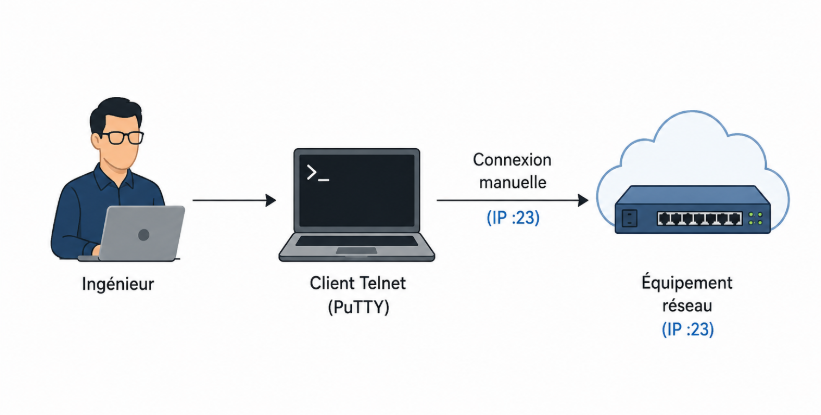
\includegraphics[width=0.88\textwidth]{images/systeme_existant}
  \caption{Schéma du processus de tests Telnet existant}
  \label{fig:systeme_existant}
\end{figure}

\subsection{Analyse critique de l'infrastructure actuelle}

\begin{table}[H]
  \centering
  \caption{Analyse critique du système de tests existant}
  \label{tab:analyse_critique}
  \begin{tabularx}{\textwidth}{|L{3cm}|L{4.5cm}|X|}
    \hline
    \textbf{Aspect} & \textbf{État actuel} & \textbf{Impact métier} \\
    \hline
    Connexion Telnet &
      Ouverture manuelle via PuTTY ou terminal &
      Risque élevé d'erreurs de saisie~; temps de connexion non optimisé \\
    \hline
    Supervision &
      Inexistante~; contrôle visuel uniquement &
      Aucune détection proactive des anomalies~; pannes non tracées \\
    \hline
    Scalabilité &
      Un seul test à la fois, un seul slot &
      Allongement des cycles de validation~; blocage des livraisons \\
    \hline
    Pipeline CI/CD &
      Absent~; déploiement manuel &
      Délais de mise en production importants~; risque de régression \\
    \hline
    Qualité et standardisation &
      Procédures non formalisées~; dépendance aux individus &
      Résultats non reproductibles~; difficulté d'audit \\
    \hline
    Reporting &
      Fichiers Excel manuels &
      Aucune centralisation~; données inutilisables pour l'analyse \\
    \hline
  \end{tabularx}
\end{table}

\noindent\textbf{Analyse des causes racines~:}
\begin{itemize}
  \item \textbf{Aucun outil dédié~:} il n'existait pas de plateforme
        conçue spécifiquement pour gérer des connexions Telnet multi-slots~;
  \item \textbf{Processus non industrialisé~:} aucune intégration dans
        une chaîne CI/CD~;
  \item \textbf{Données dispersées~:} configuration, commandes et résultats
        n'avaient pas de référentiel commun~;
  \item \textbf{Gestion des utilisateurs absente~:} ni contrôle d'accès,
        ni traçabilité des actions.
\end{itemize}

\subsection{Solution proposée}

La solution \textbf{Telnet Test Manager} couvre l'ensemble de ces
lacunes à travers trois composants principaux~:

\begin{enumerate}
  \item \textbf{Application web fullstack}
    \begin{itemize}
      \item Interface React~18/TypeScript pour la configuration et
            l'exécution des tests~;
      \item Backend Node.js/Express.js structuré selon la Clean
            Architecture~;
      \item Base de données MongoDB pour la persistance.
    \end{itemize}

  \item \textbf{Moteur de tests Telnet automatisé}
    \begin{itemize}
      \item Exécution isolée dans des Worker Threads Node.js~;
      \item Trois modes d'exécution~: commande unitaire, séquence
            d'étapes, supervision continue~;
      \item Tests multi-slots en parallèle~;
      \item Diffusion des résultats en temps réel via WebSocket.
    \end{itemize}

  \item \textbf{Infrastructure DevOps}
    \begin{itemize}
      \item Conteneurisation Docker avec build multi-stage pour
            le frontend~;
      \item Orchestration Kubernetes via chart Helm v0.3.0~;
      \item Autoscaling horizontal (HPA~: 1 à 5 répliques, seuil
            CPU à 70\,\%)~;
      \item Pipeline GitHub Actions en 3 jobs~: CI backend, CI
            frontend, déploiement~;
      \item Supervision Prometheus/Grafana avec 10 panneaux de
            métriques.
    \end{itemize}
\end{enumerate}

% -----------------------------------------------------------------
\section{Contexte et objectifs du projet}

\subsection{Contexte et historique}

Le besoin est venu directement du département d'ingénierie des tests
de Sagemcom Ezzahra. Avec la multiplication des familles de produits
--- passerelles xDSL, VDSL2, fibre, décodeurs IPTV --- et l'augmentation
du nombre de slots à valider par équipement, le processus manuel est
devenu difficile à tenir. Une première tentative basée sur des scripts
Python avait été envisagée, puis abandonnée par manque de centralisation
et d'interface utilisateur. Le projet s'est alors orienté vers une
application web moderne, évolutive et intégrée dans l'écosystème DevOps
existant.

\subsection{Méthodologie de travail}

\subsubsection{Mise en \oe{}uvre de la méthodologie Agile Scrum}

Le projet s'appuie sur la méthodologie \textbf{Agile Scrum} pour piloter
cette initiative d'automatisation. Cette approche apporte la flexibilité
et la capacité de livraison itérative nécessaires pour un projet de cette
complexité technique.

\paragraph{Apports du cadre Scrum~:}
\begin{itemize}
  \item \textbf{Livraison itérative~:} chaque composant d'infrastructure
        (moteur Telnet, conteneurisation, orchestration, CI/CD) est livré
        de façon incrémentale~;
  \item \textbf{Validation continue~:} chaque couche d'automatisation est
        vérifiée avant de passer à la suivante~;
  \item \textbf{Visibilité claire~:} toutes les parties prenantes suivent
        l'avancement en temps réel~;
  \item \textbf{Gestion des risques~:} les problèmes techniques ---
        compatibilité Docker, configuration Kubernetes, intégration
        WebSocket --- sont détectés et traités tôt~;
  \item \textbf{Alignement métier~:} les exigences techniques restent en
        phase avec les objectifs du projet tout au long du développement.
\end{itemize}

\paragraph{Structure des sprints~:}
\begin{itemize}
  \item \textbf{Durée~:} 2 semaines, adaptées aux cycles de livraison
        d'infrastructure~;
  \item \textbf{Sprint Planning~:} priorisation du backlog technique et
        allocation des ressources~;
  \item \textbf{Daily Scrums~:} synchronisation quotidienne et
        identification des blocages~;
  \item \textbf{Sprint Reviews~:} démonstration des livrables et retours
        des encadrants~;
  \item \textbf{Rétrospectives~:} amélioration continue du processus à
        chaque itération.
\end{itemize}

\begin{figure}[H]
  \centering
  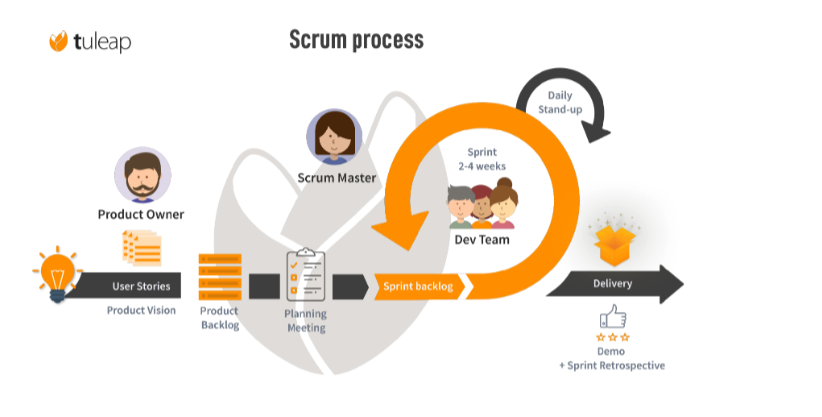
\includegraphics[width=0.88\textwidth]{images/scrum_process}
  \caption{Schéma du cadre Scrum appliqué au projet Telnet Test Manager}
  \label{fig:scrum_schema}
\end{figure}

Le schéma Scrum illustre le flux de travail complet adapté au projet.
Les sprints de deux semaines intègrent la gestion du backlog
d'infrastructure, la planification technique et les livrables. Les
Daily Scrums assurent la coordination entre les tâches DevOps,
l'implémentation de la sécurité et le développement des modules
applicatifs.

\subsubsection{Composition de l'équipe Scrum}

L'équipe est structurée pour répondre à la complexité technique et aux
exigences pluridisciplinaires du projet. Chaque rôle apporte une
expertise ciblée, dans un fonctionnement collaboratif orienté vers la
livraison d'une plateforme de tests prête pour la production.

\begin{table}[H]
  \centering
  \caption{Membres de l'équipe Scrum}
  \label{tab:equipe_scrum}
  \begin{tabularx}{\textwidth}{|L{2.8cm}|L{3.5cm}|X|}
    \hline
    \textbf{Rôle} & \textbf{Membre} & \textbf{Responsabilités principales} \\
    \hline
    Product Owner &
      Walid Ncir\newline\textit{(Encadrant Sagemcom)} &
      Définition des exigences métier, priorisation du backlog produit,
      validation des livrables et alignement avec les objectifs de
      l'équipe tests de Sagemcom Ezzahra \\
    \hline
    Scrum Master &
      Rim Tlili\newline\textit{(Encadrante académique)} &
      Facilitation du processus Scrum, levée des obstacles,
      application de la méthodologie agile et suivi de l'avancement
      académique du projet \\
    \hline
    Équipe de développement &
      Adem Hmercha\newline\textit{(Étudiant PFE)} &
      Conception de l'architecture système, développement fullstack
      (Node.js, React, MongoDB), implémentation du moteur Telnet et
      déploiement de l'infrastructure DevOps complète \\
    \hline
  \end{tabularx}
\end{table}

\section{Conclusion}

Ce chapitre a posé les bases nécessaires à la mise en place d'une
plateforme de tests Telnet automatisée et orientée DevOps au sein de
\textbf{Sagemcom Ezzahra}. L'analyse menée montre clairement où se
situent les manques~: automatisation absente, supervision inexistante,
traçabilité insuffisante --- autant de points qui ralentissent le
département et allongent les délais de livraison des firmwares validés.

La solution \textbf{Telnet Test Manager} répond à ces problèmes par
une approche DevOps structurée~: moteur d'exécution Telnet automatisé,
supervision temps réel via WebSocket, gestion centralisée des équipements
et pipeline CI/CD de bout en bout. Passer des opérations manuelles à une
plateforme automatisée, ce n'est pas juste une mise à jour technique ---
c'est une façon différente de travailler pour toute l'équipe d'ingénierie
des tests.

Avec une automatisation complète et une supervision en temps réel,
Sagemcom Ezzahra gagne en fiabilité, en traçabilité et en efficacité
sur la validation de ses équipements réseau embarqués. La méthodologie
\textbf{Agile Scrum} encadre cette transition en découpant la livraison
en sprints de deux semaines, chacun avec des critères de succès clairs,
ce qui permet de garder le contrôle sur la qualité, la sécurité et les
performances à chaque étape.

Cette analyse prépare les phases d'implémentation qui suivent, en fixant
des attentes précises sur les livrables, les délais et les métriques à
atteindre. L'architecture retenue --- Clean Architecture, WebSocket,
Docker, Kubernetes, GitHub Actions --- forme une base solide pour une
plateforme de tests durable et évolutive.

Au final, la réalisation de cette plateforme DevOps permettra à l'équipe
d'ingénierie de Sagemcom Ezzahra de valider ses firmwares embarqués plus
vite, avec une meilleure traçabilité et une productivité accrue ---
que ce soit avec la version actuelle de Telnet Test Manager ou ses
évolutions futures.

